\documentclass[9pt]{beamer}


\usepackage{introLatex}
\usepackage{shortcutLatex}
\usepackage{layout}
\usepackage{algorithm}
\usepackage{algorithmic}


% Dossier où se trouvent les images
\graphicspath{{imagesdiapo/}}


\newcommand{\widesim}[2][1.5]{
  \mathrel{\underset{#2}{\scalebox{#1}[1]{$\sim$}}}
  }

\newcommand*{\sepfbox}[1]{%
  \begingroup
    \sbox0{\fbox{#1}}%
    \setlength{\fboxrule}{0pt}%
    \fbox{\kern-\fboxsep\fbox{\unhbox0}\kern-\fboxsep}%
  \endgroup
}

\begin{document}

	\begin{frame}[t]
	\titlepage
	\end{frame}


	\begin{frame}
	\vspace*{22pt}
	\tableofcontents
	\end{frame}





\footHeadLine{}

\section{Introduction du problème}

\subsection{Physique statistique et modèle d'Ising}

\setlength{\columnseprule}{0.4pt}
\begin{frame}
		\justifying
		\vspace*{22pt}


\begin{multicols}{2}

		$\bullet$ Modèle d'Ising 2D carré :
			$N_s$ spins à une composante sur un quadrillage
			\vspace*{-11pt}
			
\begin{figure}[H]
\begin{center}
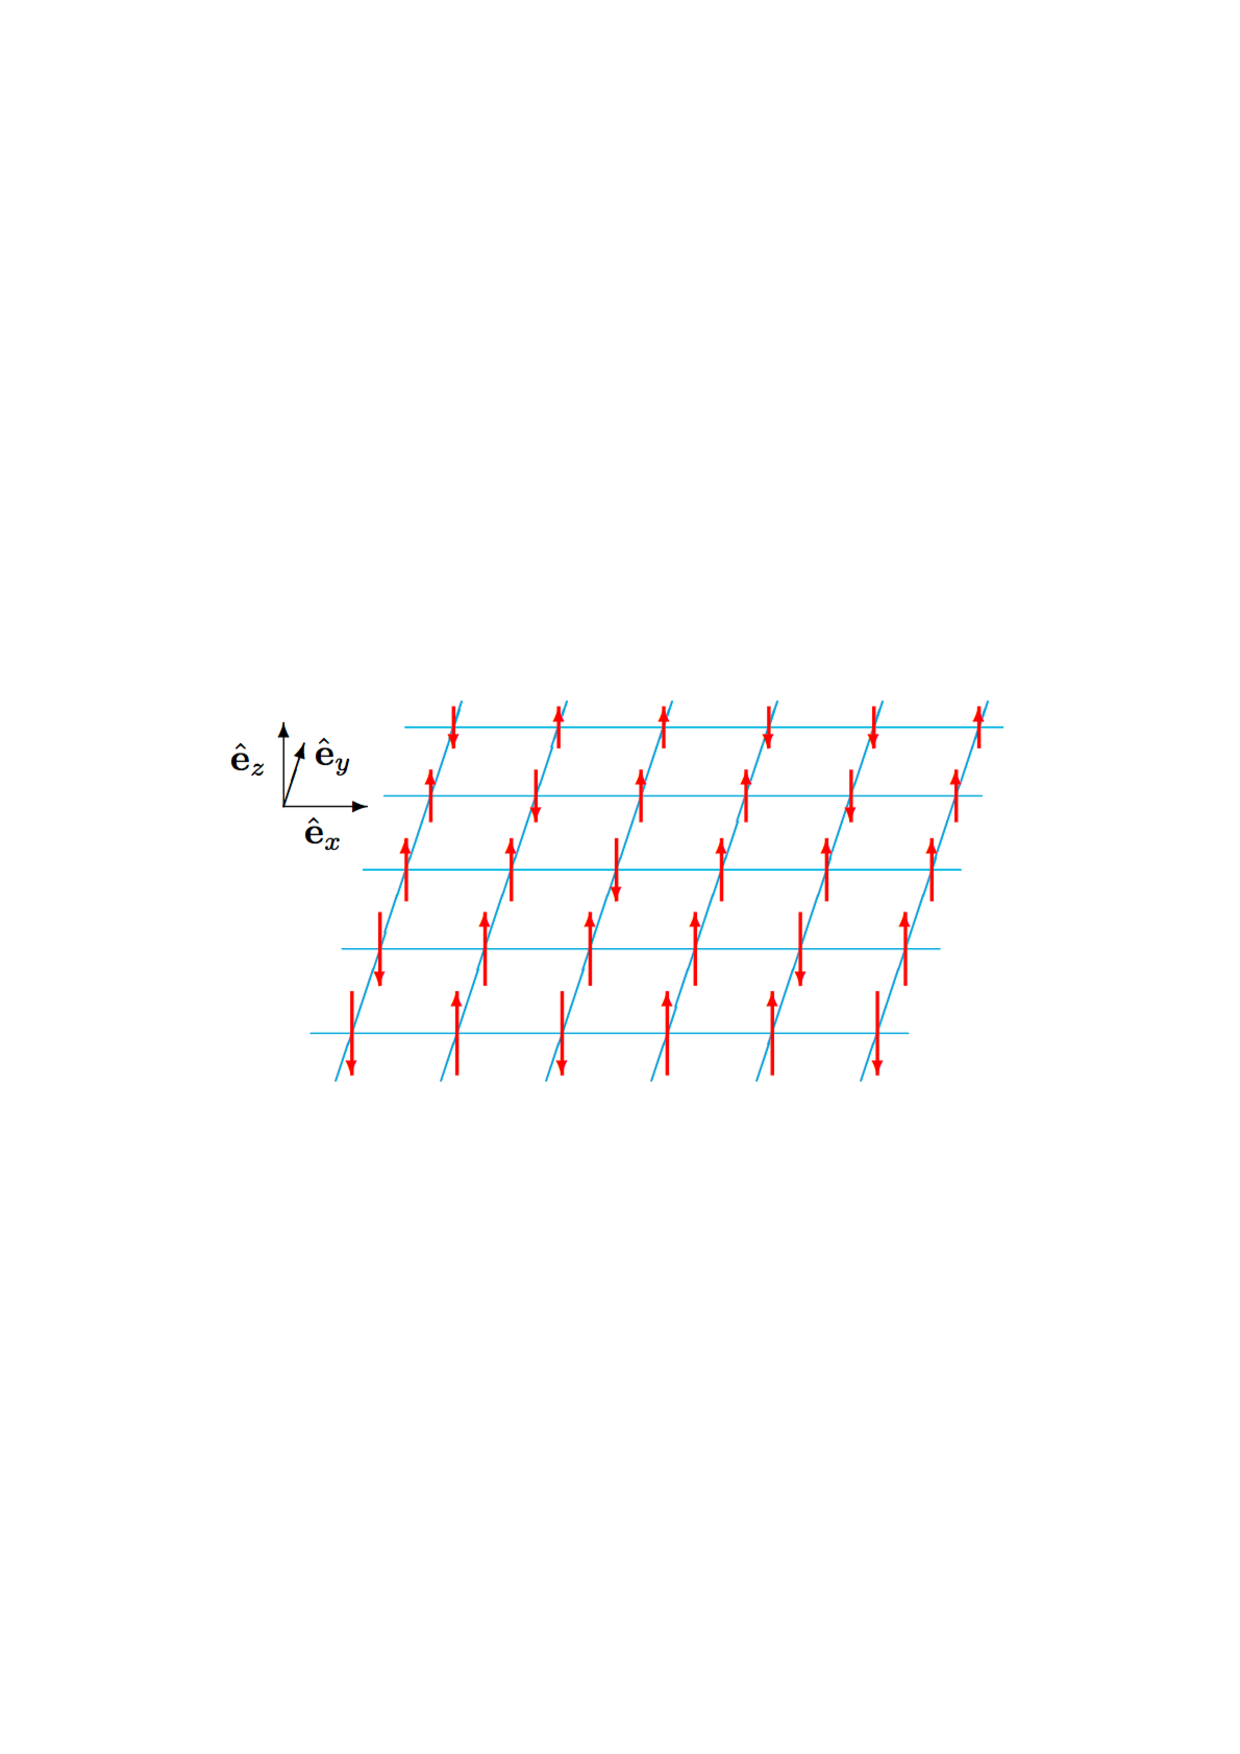
\includegraphics[scale =0.35]{Ising2D.pdf}
\caption{Modèle d'Ising.}
	\label{fig:schemaIsing}
	\end{center}
\end{figure}

$\bullet$ Spin et configuration :
\begin{equation*}
 S_\rv \ = -1(\downarrow), +1(\uparrow), \quad \Mr = \{S_\rv\}_\rv
\end{equation*}


$\bullet$ Energie d'une config. $\Mr$ : $ \Hc(\Mr,b)$ \\
\commentout{\begin{equation*}
  \Hc(\Mr) = \sum_{\left< \rv, \rv' \right>} S_\rv S_{\rv'} - \sum_\rv b_\rv S_\rv	
\end{equation*}}

\vspace*{11pt}
$\bullet$ Probabilité d'une config. $\Mr$ :
\begin{equation*}
p(\Mr,b, T) = \frac{1}{\Zc(b,T)} \exp\(-\frac{\Hc(\Mr,b)}{k_BT}\)
\end{equation*}
$\bullet$ Fonction de partition :
\begin{equation*}
\Zc(b,T) = \sum_\Mr \exp\(-\frac{\Hc(\Mr,b)}{k_BT}\)
\end{equation*}
\vfill

	\end{multicols}
\end{frame}

\begin{frame}
		\justifying
		\vspace*{22pt}
	$\bullet$	Définition de l'aimantation :  
		\begin{equation*}
			m(T,b) = \sum_{\Mr = \{S_\rv\}_\rv }  \left\{p(\Mr,b,T) \( \frac{1}{N_s} \sum_\rv S_\rv\) \right\}  \propto \partial_T \ln\(\Zc \) 
		\end{equation*}
		
	\onslide<2->{	
		\vspace*{11pt}
		$\bullet$ Evolution de l'aimantation $m(T,b=0)$ avec la température $T$ :
		
\begin{multicols}{2}


	\begin{figure}[H]
\begin{center}
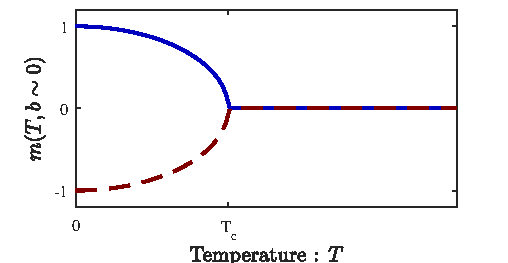
\includegraphics[width =0.95\columnwidth]{aimantation.pdf}
\caption{Aimantation $m$ vs $T$ à $b \sim 0$}
	\label{fig:schemaIsing}
	\end{center}
\end{figure}
	
	\vspace*{-11pt}
	Invariance par échange de $\ev_z$ en $-\ev_z$ :\\
	$\Hc(\Mr,b=0) = \Hc(-\Mr,b=0)$ \\
	$\quad \diamond$ symétrie $\mathbb{Z}_2$ \\
	$\quad \diamond$  $m(b = 0, T=0)=0$. \\
	\vspace*{8pt}}
	\onslide<3->{
	Mais problème : 
	\begin{equation*}
		\lim_{N_s \to \infty} \(\lim_{b \to 0} m \) = 0 \neq \lim_{b \to 0} \( \lim_{N_s \to \infty} m \)
	\end{equation*}
	
	\end{multicols}
	}
	\onslide<4->{
	\begin{center}
$\Rightarrow$ {\Large Brisure de symétrie \& Transition de phase }
\end{center}
		}
\end{frame}
    



\commentout{
\subsection{Transition de phase}

	\begin{frame}
		\justifying
		\vspace*{22pt}


\onslide<1->{$\bullet$ Température critique : $T_c$} \\

\vspace*{11pt}
\onslide<2->{$\bullet$ Transitions de phase du second ordre : \\


$\quad \diamond$ Fonction de corrélation à deux points :
\begin{equation*}
\begin{split}
	G^{(2)}(|\rv_1 - \rv_2|) & \equiv \left< S_{\rv_1} S_{\rv_2} \right>   \equiv \sum_{\Mr}  p\(\Mr\) S_{\rv_1} S_{\rv_2} \, 
	\end{split}
\end{equation*}
$\quad \diamond$ Longueur de corrélation $\xi$ : 
\begin{equation*}
G^{(2)}(r >\xi) \simeq 0 \quad \text{et} \quad G^{(2)}(r < \xi) \neq 0
\end{equation*}
\vspace*{2pt}
}

\onslide<3->{
$\bullet$ Exposants critiques $\eta$ et $\nu$ :
\begin{equation*}
	\xi \widesim{T \to T_c} |T-T_c|^{-\nu} \quad \text{et à } T = T_c, \quad	 G^{(2)}(r) \widesim{r \to \infty} |r|^{2-d-\eta}
\end{equation*}

}

\onslide<4->{
\begin{center}
$\Rightarrow$ {\Large Universalité des exposants critiques }
\end{center}
}

	\end{frame}
}

\setlength{\columnseprule}{0pt}


\commentout{
	\begin{frame}
		\justifying
		\vspace*{22pt}

$\bullet$ Fonction de partition exprimée avec des champs :
\begin{equation*}
	\Zc = \int \Dc \varphiv \exp\(-\Hc[\varphiv]/(k_BT)\)
\end{equation*}


\begin{multicols}{2}

$\bullet$ Transformée de Fourier :
\vspace*{-11pt}
\begin{equation*}
\begin{split}
\hat{\varphiv}_\pv = \frac{1}{\sqrt{|\Omega|}}\int_\Omega \varphiv(\rv) \, e^{-i \pv . \rv} \dd \, \rv, \\
\varphiv(\rv) = \frac{1}{\sqrt{|\Omega|}}\sum_\pv \hat{\varphiv}_\pv \, e^{i \pv  .\rv}
\end{split} 	
\end{equation*}
$ \bullet $ $\|\pv \|_2 \in [0, \Lambda]$
\vspace*{22pt}
\begin{figure}
\begin{center}
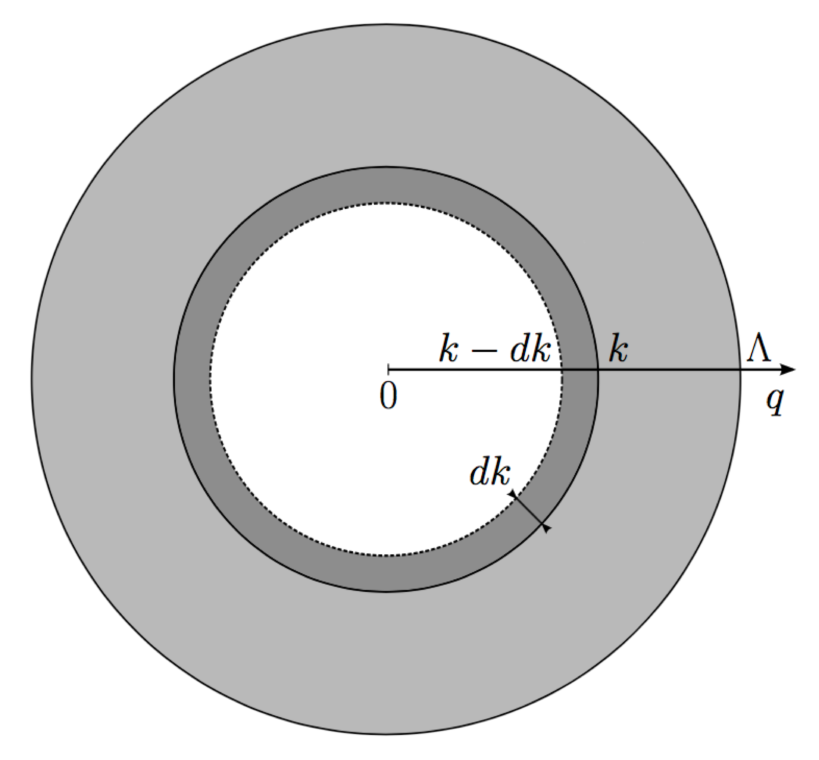
\includegraphics[scale = 0.3]{SchemaRG.pdf}
\caption{Principe du RG \\ {\footnotesize \textit{Thèse de Frédéric Léonard}}}
	\label{fig:SchemaRG}
	\end{center}
\end{figure}

\end{multicols}

	$\bullet$ En pratique :  $\Zc_k \underset{\text{NPRG}}{\longrightarrow} \Gamma_k   \underset{\text{BMW}}{\longrightarrow} \Gamma^{(2)}_k$
	\end{frame}
	
}

    
    \subsection{Objectifs de l'étude}
    \begin{frame}
		\justifying
		\vspace*{22pt}
    
    %\onslide<1->{$\Rightarrow$ {\Large Calcul des exposants critiques : $\eta$ et $\nu$ } }\\
    \onslide<1->{$\Rightarrow$ {\Large Calcul de la température critique : $T_c$ \\}
   	$\Rightarrow$ {\Large Calcul des exposants critiques} } \\
   	
   	
   	
   	
   	
   	\vspace*{11pt}
    \onslide<2->{
    $\rightarrow$ Méthode : calcul de la fonction de partition $\Zc$\\
    $\rightarrow$ Utilisation du NPRG\\
    $\rightarrow$ Utilisation de l'approximation BMW \\
    $\rightarrow$ Benchmarking de l'approximation BMW \\}
    \vspace*{11pt}
    

\commentout{
    \onslide<3->{
    $\bullet$ Première étude :\\
    \begin{itemize}
    \item Réecriture en C++ d'un code de calcul des exposants critiques
    \item Recherche des problèmes et tentatives de résolution
    \end{itemize}
    }
    }
    \vspace*{11pt}
    
    \onslide<3->{
    $\bullet$ Deuxième étude :\\
    \begin{itemize}
    \item Ecriture d'un nouveau code pour calculer $T_c$.
    \item Comparaison à la valeur théorique : benchmarking de la méthode
    \end{itemize}
    }
    
    \end{frame}

    
 \commentout{   

    
    \section{Le problème continu}
    \subsection{Hamiltonien du modèle continu $\varphiv^4$}
    
        \sommaire{}
    
    
      \begin{frame}
		\justifying
		\vspace*{22pt}
    
    \begin{equation}
		H[\varphiv] = \int_\rv \, \left\{ \frac{1}{2}(\nabla \varphiv)^2 + \frac{1}{2}r_0 \varphiv^2 + \frac{u_0}{4!}{\({\varphiv}^{2}\)}^{2} \right\}
		\label{eq:hamiltCont}
\end{equation}
    	\end{frame}
    
    
    \subsection{Système d'équations à résoudre}
    
    
    \begin{frame}
		\justifying
		\vspace*{22pt}

{\itshape Trouver $(\tY_k,\tW_k)$ tel que pour tout $k \in ]0 ,\Lambda]$,  $\trho \in [0, +\infty[$ et $\tp \in [0, +\infty[$,}
\begin{align*}
	\partial_t  \tY_k(\tp, \trho) & = 
	\begin{aligned}[t]
			& \eta_k(1+\tY_k(\tp, \trho)) + \tp \, \partial_{\tp} \tY_k(\tp, \trho)  -(2-d-\eta_k)\trho \,\partial_{\trho} \tY_k(\tp, \trho)  \quad  \\
			& + 2\trho \tp^{-2} \left[ {\( \tp^2 \partial_{\trho} \tY_k(\tp, \trho) + \tilde{u}_k(\trho)\)}^2\, \tJ_3(\tp, \trho) \right]  - 2\trho \tp^{-2} \left[ \tilde{u}_k^2(\trho)  \tI_3(\trho) \right] \\
			&  - \tI_2(\trho) \(  \partial_{\trho} \tY_k(\tp, \trho) / 2 + \trho \,  \partial_{\trho}^2 \tY_k(\tp, \trho) \)
	\end{aligned}
	\label{eqn}\\
	\partial_t  \tW_k &  = 
	\begin{aligned}[t]
		& (\eta_k-2) \tW_k(\trho) + (d-2+\eta_k) \trho \,\partial_{\trho}\tW_k(\trho) + \frac{1}{2} \partial_{\trho} \tI_1(\trho) \, ,
	\end{aligned}
\end{align*}
\textit{avec la définition}
\begin{equation*}
\begin{split}
\eta_k = \frac{1}{2}  \tI_2(\trho = 0)\partial_\rho\tY_k(\tp = 0, \trho = 0) \,, 
\end{split}
\end{equation*}
\textit{et les conditions initiales,}
\begin{equation*}
	\tY_\Lambda(\tp, \trho) = 0 \quad  \text{et} \quad \tW_\Lambda(\trho) = \tilde{r}_0 + \tilde{u}_0\trho
\end{equation*}

	\end{frame}
	

	\subsection{Méthodes numériques}
	
	
     \begin{frame}
		\justifying
		\vspace*{22pt}
    
    
   	\onslide<1->{$\bullet$ Discrétisation en temps : Schéma d'Euler explicite} \\
   	\onslide<2->{$\bullet$ Discrétisation en champ : Grille fixe. Dérivée avec schémas à 5 points}\\
   	\onslide<3->{$\bullet$ Discrétisation en moments : Méthode pseudo-spectrale
   	\begin{itemize}
   		\item Interpolation de Tchebytechev	
   		\item Intégration de Gauss-Legendre
   	\end{itemize}
 } 	
   	\vspace*{11pt}
   
   \onslide<4->{	
   	$\bullet$ A propox de l'intégration
   	\begin{equation*}
K = \int_{\R^d} f(\tqv^2)g((\tpv+\tqv)^2) \, \dd \, \tqv \, ,
\end{equation*}
\begin{equation*}
K = S_{d-1} \int_0^{+\infty} \dd\tq_2 \, \tq_2^{d-2} \int_{-\infty}^{+\infty} \dd\tq_1 \, f(\tq_1^2 + \tq_2^2) g(\tp^2 + \tq_1^2 + \tq_2^2 + 2\tp\tq_1)
\end{equation*}

}
	\end{frame}
	
	
	
	\subsection{Résultats}
	
	   \begin{frame}
	\justifying
	\vspace*{22pt}

	
	
	\end{frame}
	
	}
	
	\section{Etude du modèle d'Ising 2D : Mise en équation}
    	
    	\subsection{Calcul de la fonction de partition}
    	
    	\sommaire{}
   	
	   \begin{frame}
	\justifying
	\vspace*{22pt}


$\bullet$ Calcul de $T_c$ pour le modèle d'Ising avec la méthode NPRG et l'approximation BMW. Comparaison avec le résultat du calcul exact.\\

\vspace*{11pt}


\commentout{
	
\only<1>{
	$\bullet$ Fonction de partition Ising 2D :
\begin{equation*}
\Zc = \sum_{\Mr = \{S_\rv\}_\rv} \exp\( -\frac{\Hc(\Mr,b=0)}{k_BT}\) \, ,
\end{equation*}
avec l'hamiltonien $\Hc$ définit par 
\begin{equation*}
\Hc(\Mr = \{S_\rv \}_\rv, b=0) = -J\sum_{\left<  \rv, \rv'\right>} S_\rv S_{\rv'} \quad (J > 0)
\end{equation*}
}
}

\only<1->{	
$\bullet$ Réécriture de la fonction de partition : 
	\begin{equation*}
  \Zc  \propto \int \prod_{\rv} \, \dd \varphi(\rv) \, \exp\(-\Hc[\varphi] \) \, ,
\end{equation*}

avec $\varphi \in \Cc^0(\R^2)$ et l'hamiltonien $\Hc$ défini par 
\begin{equation*}
  \Hc[\varphi] = \frac{1}{2} \int_\qv \hat{\varphi}(\qv) \frac{1}{\lambda(\qv)} \hat{\varphi}(-\qv) - \sum\limits_\rv \ln\(\cosh(\varphi(\rv))\) \, ,
\end{equation*}

avec $\lambda$ une fonction $\Cc^\infty$ et la notation
\begin{equation*}
\int_\qv ... \, \equiv \, \int_{-\pi}^{\pi}	\int_{-\pi}^{\pi}	... \, \dd \, q_x \dd \, q_y \, .
\end{equation*}
$\bullet$ Avec cette notation $\Hc$ dépend de la température $T$.
}

	
	\end{frame}
	
	
	
	\subsection{Le NPRG et les équations BMW}

	\begin{frame}
		\justifying
		\vspace*{22pt}
$\bullet$ L'équation de flot BMW à résoudre : \\

\sepfbox{
\begin{minipage}{300pt}
\textit{Trouver $\Gamma^{(2)}$ tel que pour tout $(\pv, \phi, t) \in [-\pi, \pi]^2 \times \R \times ]-\infty, 0]$,}  
\begin{equation*}
\begin{split}
	\partial_t \Gamma^{(2)}(t,\pv, \phi) & = J_3(t,\pv, \phi) {\( \partial_\phi \Gamma^{(2)}(t,\pv, \phi) \)}^2  - \frac{1}{2}  I_2(t,\phi) \, \partial_\phi^{2} \Gamma^{(2)}(t,\pv, \phi) \quad 
\end{split}
\label{eq:flotBMW}
\end{equation*}
\end{minipage}}
\vspace*{11pt}
\begin{minipage}[b]{300pt}
\textit{Avec les notations}
\begin{equation*}
\begin{split}
	J_n(t, \pv,\phi) & = \int_\qv \partial_t \Rc(t,\qv) \, G(t,\pv+\qv, \phi) \,G^{n-1}(t,\qv, \phi) \, , \quad \\ I_n(t,\phi) &  = J_n(t,\pv = 0,\phi). \\
G(t,\qv, \phi) & = \frac{1}{\Gamma^{(2)}(t,\qv,\phiv)+ \Rc(t,\qv)} \quad \quad \textit{(propagateur)}  \\
\Rc(t,\qv) & \in \Cc^{\infty}(\R^{3}) \qquad \qquad \qquad \qquad \quad \textit{(régulateur)} 
\end{split}
\end{equation*}
$\bullet$ Condition initiale : en $t = 0$, dépend de $\Hc$ et donc de $T$. \\
$\bullet$ Détermination de $T_c$ : calcul de $\Gamma^{(2)}$ en $t \to -\infty$

\commentout{
\\indent
$\quad \diamond$ Utilisation d'une version adimensionné de l'équation. \\
\indent
$\quad \diamond$. \\}

\end{minipage}
	\end{frame}
    
	
	
	
	
	
	
	\subsection{La résolution en trois étapes}


\commentout{
	
	\begin{frame}
	\justifying
	\vspace*{22pt}
	
	$\bullet$ Système d'équation à résoudre : \\
	\vspace*{11pt}
	{\itshape Trouver $(\Delta$, $X)$, tels que pour tout $(p_x, p_y) \in [-\pi, \pi]^2$, $\phi \in \R$, $t \in ]-\infty, 0]$}
	\begin{align*}
	\partial_t  \Delta (t,p_x, p_y, \phi) & = 
	\begin{aligned}[t]
	&  J_3(t,p_x, p_y, \phi) \partial_{\phi} \left\{ \Delta (t, p_x, p_y, \phi) + X(t,\phi) \right\} \\
	&  - \frac{1}{2} I_2(t,\phi) \partial_{\phi}^2 \Delta(t,p_x, p_y, \phi) - I_3(t,\phi){(\partial_{\phi} X(t,\phi))}^2 \quad \quad (\Ec_1)
	\end{aligned}
	\label{eqn} \\
	\partial_t X(t,\phi) & = 
	\begin{aligned}[t]
		& \frac{1}{2} \partial_{\phi}^2 I_1(t,\phi) \, ,
	\end{aligned}
\end{align*}
\textit{avec la condition intiale}
	\begin{equation*}
	\Delta(0,p_x, p_y, \phi) = 0 \quad \text{et} \quad X(0,\phi) =  \delta^2 \frac{1}{1+\tilde{\mu}} - \frac{2\delta^2\tilde{\beta} }{\cosh^2\(\delta\sqrt{2\tilde{\beta}}\phi\)}
\end{equation*}
	
	
	\end{frame}
	}
	
	
	\begin{frame}
	\justifying
	\vspace*{22pt}
	
	$\bullet$ Problème :
	
	\begin{figure}[H]
\begin{center}
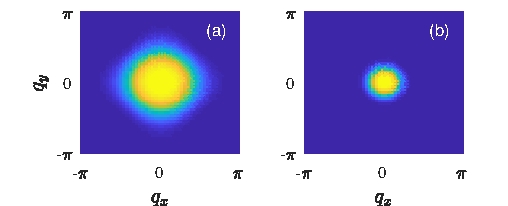
\includegraphics[scale = 0.9]{DerRegIsing.pdf}
\caption{Représentation de $\partial_t \Rc(t_1, q_x, q_y)$, $\partial_t \Rc(t_2, q_x, q_y)$, avec $t_2 < t_1$}
	\label{fig:schemaIsing}
	\end{center}
\end{figure}
\vspace*{-5pt}
\begin{equation*}
	I_n, \, J_n \propto \int_{-\pi}^{\pi}\int_{-\pi}^{\pi} \partial_t \Rc(t, q_x, q_y) \times ... \dd q_x \dd q_y
\end{equation*}

$\bullet$ Changement de système d'équation (pour $t<t_a$) :\\
$\quad$ Utilisation des variables $\tqv = e^{-t}\qv = (e^{-t}q_x, e^{-t}q_y)$ \\
\vspace*{8pt}
	
	
	$\bullet$ Changement de système d'équation (pour $t<t_b< t_a$) :\\
$\quad$ Passage à un système d'équations totalement adimensionné. \\
$\quad$ Recherche d'une solution particulière dite "de point fixe".

	
		\end{frame}
	
	\section{Etude du modèle d'Ising 2D : Méthodes numériques}
	\subsection{Discrétisation en temps et en champs}
	
	\sommaire{}
	
	\begin{frame}
	\justifying
	\vspace*{22pt}
	
	Objectif : discrétiser et faire des calculs sur des fonctions
	\vspace*{-5pt}
	\begin{center} 
	$(t, q_x, q_y, \phi) \to f(t,q_x, q_y, \phi)$	
	\end{center}

	
	\vspace*{11pt}

	$\bullet$ Discrétisation en temps $t$ : \\
	$\quad \diamond$ Grille de points $\{t_n\}_n$ régulièrement espacés.\\
	$\quad \diamond$  Schéma d'Euler explicite : $\partial_t f(t, ...) = \(f(t_n, ...)- f(t_{n-1}, ...)\)/\delta t$ \\
	
	\vspace*{11pt}
	
	$\bullet$ Discrétisation en champ $\phi$: \\
	$\quad \diamond$ Grille de points $\{\phi_n\}_n$ régulièrement espacés. \\
	$\quad \diamond$ Calcul des dérivées $\partial_\phi f(..., \phi)$ avec des schémas à 5 points. \\
	
	\vspace*{11pt}
	\begin{figure}[H]
	\begin{center}
		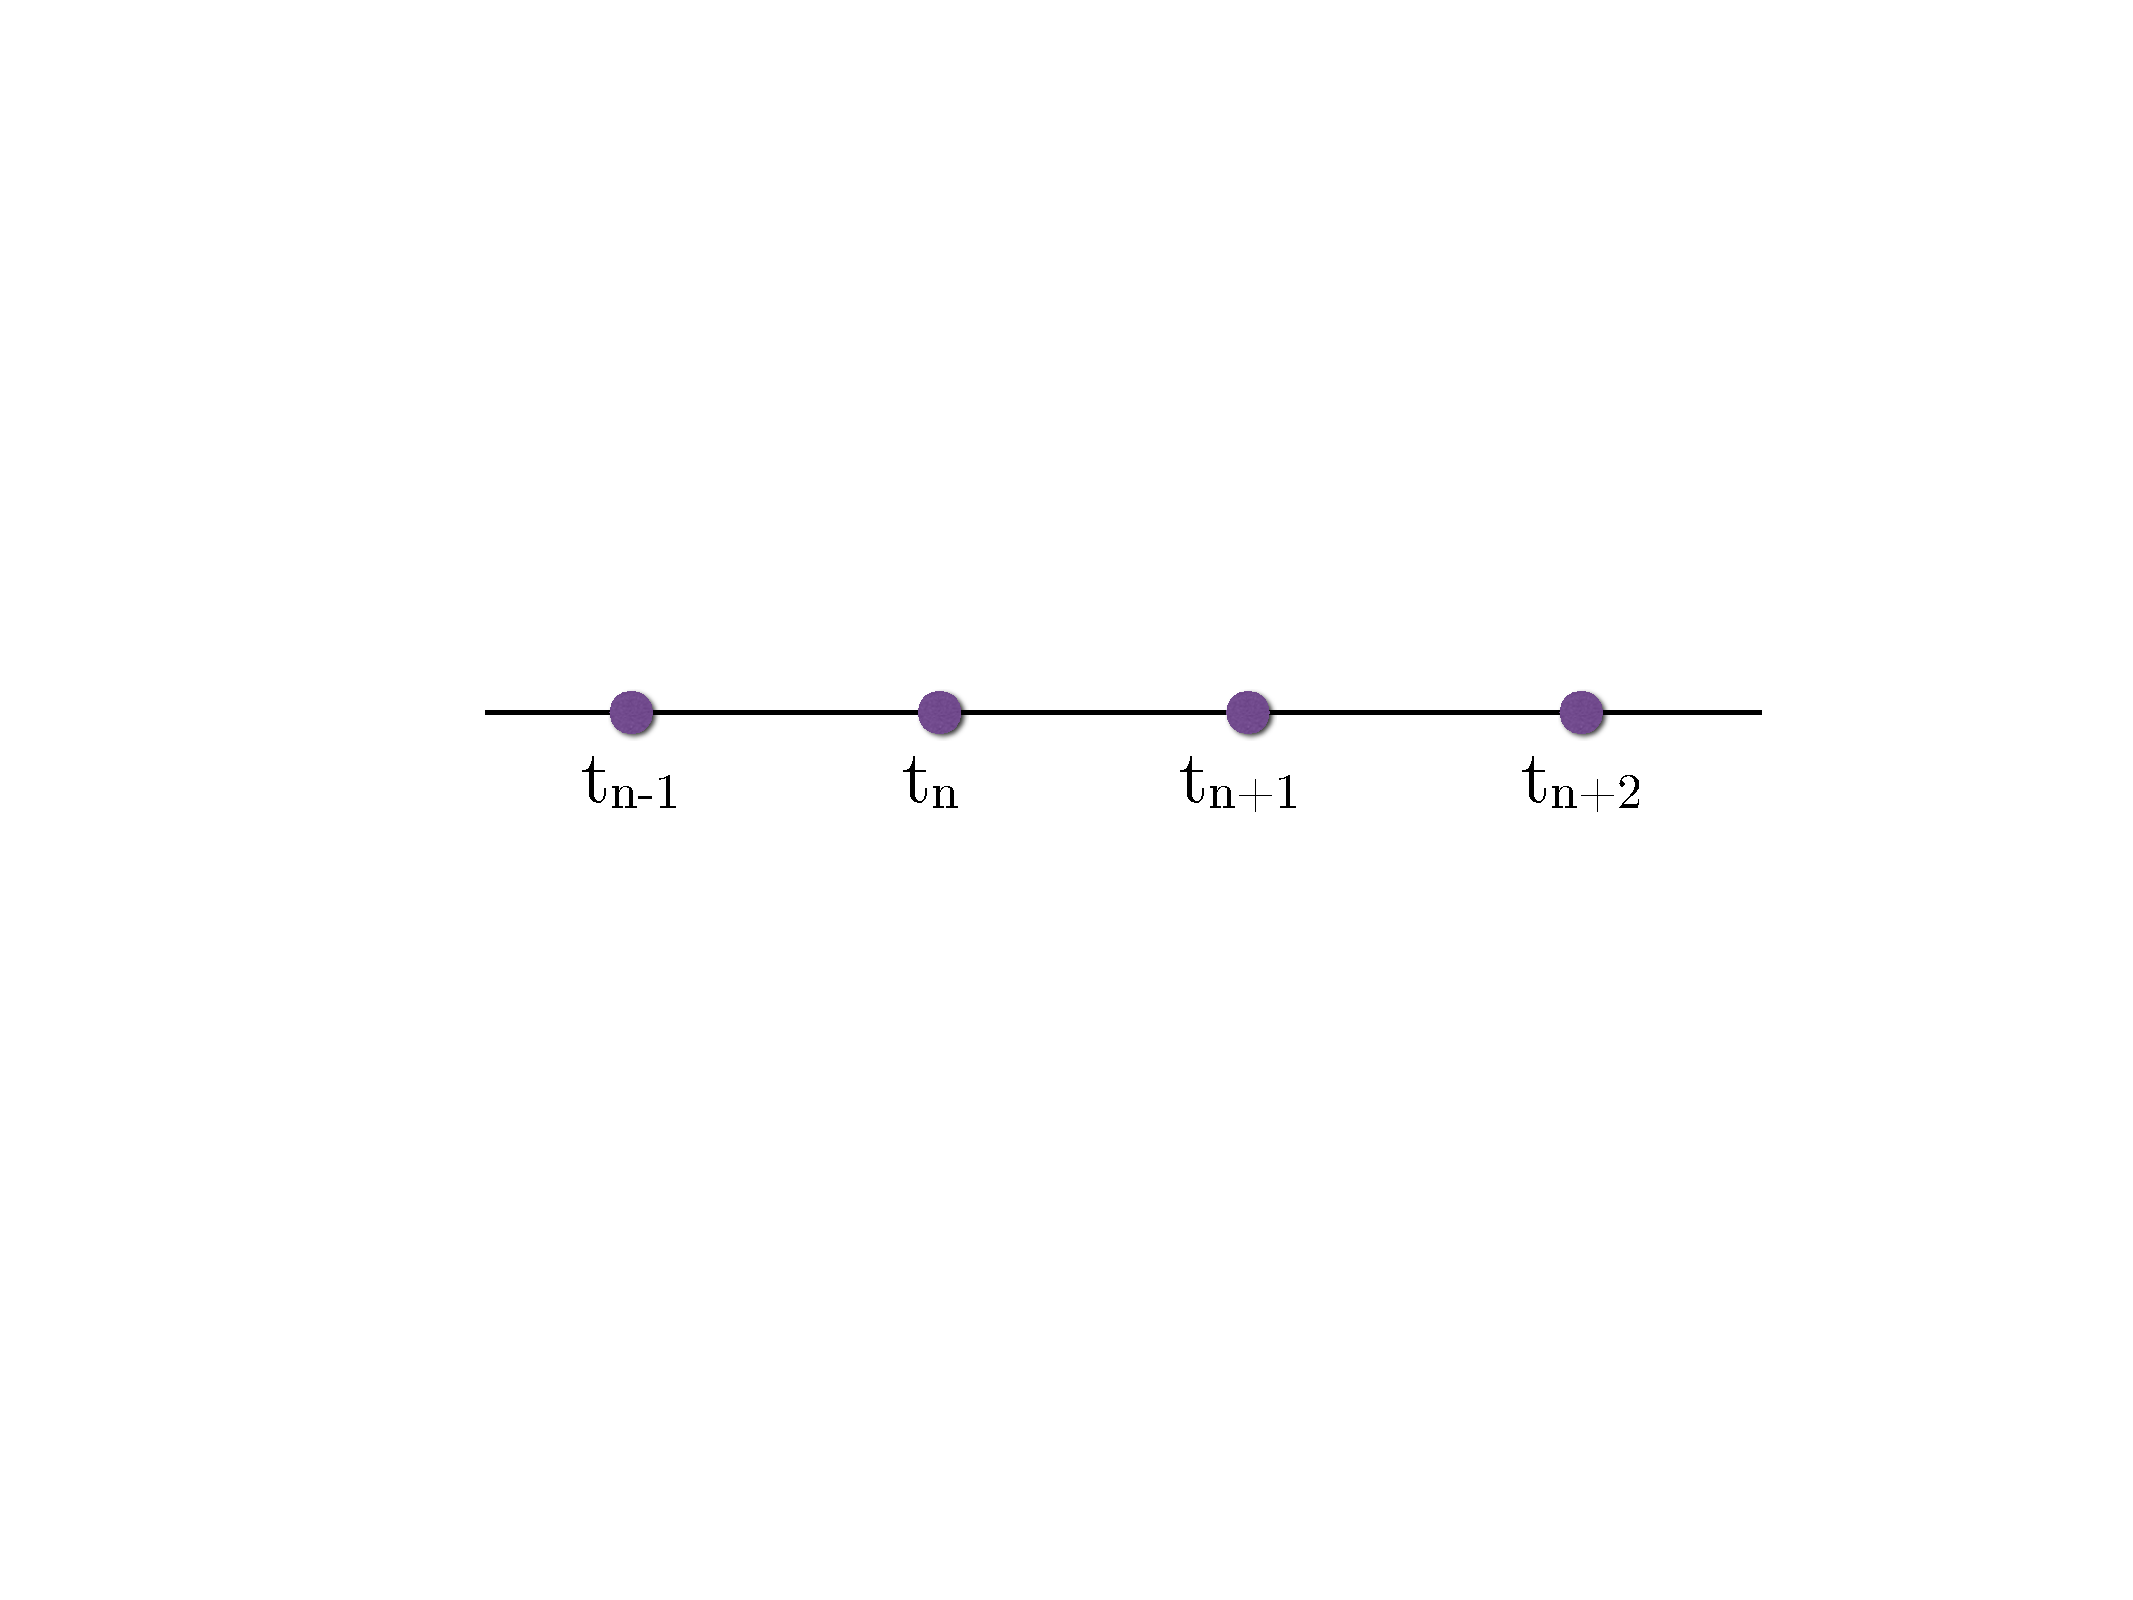
\includegraphics[scale = 0.32]{LigneTn.pdf}
	\label{fig:schemaIsing}
	\end{center}
\end{figure}
		
	
	\end{frame}
	
		
	\subsection{Intégration de Gauss Legendre}
	
	
	\begin{frame}
	\justifying
	\vspace*{22pt}
	
	$\bullet$ Calcul des intégrales : quadrature de Gauss-Legendre \\
	$\quad \diamond$ On cherche à calculer : 
	
	\begin{equation*}
		K(t,\phi) = \int_{-a}^{a} \int_{-a}^{a} f(t, q_x, q_y,\phi) \dd q_x \, \dd q_y 
	\end{equation*}
	$\quad \diamond$ Utilisation de $\{\xi_i\}_i$ points d'intégrations de Gauss-Legendre (zéros du polynômes de Legendre d'ordre $n_{gl}$) sur $[-1,1]$ et $\{w_i\}_i$ les poids associés :
	\begin{equation*}
		K(t, \phi) \simeq a^2 \sum_{i=1}^{n_{gl}} \sum_{j=1}^{n_{gl}} w_i w_j f(t,a\xi_i, a\xi_j,\phi) 
	\end{equation*}
	$\quad \diamond$ Utilisation des symétries des fonctions pour réduire les calculs.
	
	\vspace*{11pt}
	$\bullet$ Problème : le calcul de $J_n(t,p_x, p_y,\phi)$ = $\int g(t,p_x+q_x, p_y+q_y, \phi)$\\
		$\quad \diamond$ On ne connait $g$ qu'au point de discrétisation des fonctions inconnues.\\
		$\quad \diamond$ Si $q_x = a\xi_i$ et $p_x = a\xi_j$, générallement $p_x+q_x \neq a\xi_m$ $\forall m \in \bbrac{1, n_{gl}}$
	

	
	\end{frame}
	
	\vspace*{11pt}
	

	
	\subsection{Interpolation de Tchebytchev}
	
	\begin{frame}
	\justifying
	\vspace*{22pt}
	
	$\bullet$ Interpolation de Tchebytchev en deux dimensions : \\
	
	\vspace*{11pt}
	
	
	\only<1>{Soit $f$ une fonction de deux variables de $[a,b]^2$ dans $\R$. On note $\{x_n\}_{n \in \bbrac{1,n_c}}$ l'ensemble des $n_c$ racines du polynôme de Tchebytchev d'ordre $n_c$. \\
	\vspace*{8pt}
	On introduit : 
	
\begin{equation*}
	\mat{F} = \( \(  f\(\frac{a+b}{2} + x_m\frac{b-a}{2}, \frac{a+b}{2} + x_n\frac{b-a}{2}\)     \)  \)_{m,n} 
\end{equation*}

\vspace*{8pt}
$\Rightarrow$ Approximation de rang faible de cette matrice

}	
	\only<2>{
	
	Algorithme d'approximation par élimination Gaussienne
	
	\begin{algorithm}[H]
  \begin{algorithmic}[1]
    \STATE Initialisation : $\mat{E}^0 = \mat{F}$; $\mat{F}_0 = 0$; $k = 1$;
    \WHILE{ ${\| \mat{E}^k \|}_{\infty} < \varepsilon {\| \mat{E}^0 \|}_{\infty}$ }
    \STATE $(i_k, j_k) =  {\text{argmax}}_{(i,j)} \left\{\left| \mat{E}^{k-1}_{i,j} \right| \right\}$
    \STATE $\mat{C}^k_{j} = \mat{E}^k_{i_k,j}$;  $\mat{R}^k_{i} = \mat{E}^k_{i,j_k}$; $d_k = \mat{E}^k_{i_k,j_k}$
    \STATE $\mat{E}^k_{i,j} = \mat{E}^{k-1}_{i,j} - d_k^{-1}\mat{C}^k_{j}\mat{R}^k_{i}$
    \STATE $\mat{F}^k_{i,j} = \mat{F}^{k-1}_{i,j} + d_k^{-1}\mat{C}^k_{j}\mat{R}^k_{i}$
    \ENDWHILE
  \end{algorithmic}
\end{algorithm}

  \vspace*{-15pt}
\begin{equation*}
\mat{F} \simeq \sum_{j=1}^Q d_j \mat{C}^j \mat{R}^j \Rightarrow 
f(x,y) \simeq \sum_{j=1}^Q d_jc^j(y)r^j(x)
\end{equation*}

}
	
	\end{frame}
	

		
		\section{Etude du modèle d'Ising 2D : Résultats}
		\sommaire{}
		\begin{frame}
	\justifying
	\vspace*{22pt}
	
	\begin{figure}[H]
\begin{center}
	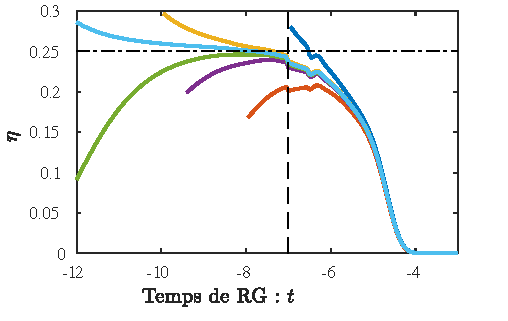
\includegraphics[scale=0.7]{MesuRes.pdf}
\end{center}
\caption{Évolution de $\eta_k$ en fonction de $t$ pour différentes valeurs de la températue $T$.}
\label{fig:etaMesu}
\end{figure}

$\bullet$ Encadrement de la température critique
\begin{equation}
2.350  < T_c^{BMW}  < 2.375 
\end{equation}

$\bullet $ Comparaison à la température théorique attendue $T_c^{th} \simeq 2.269$
\begin{equation}
	err = \frac{ |T_c^{BMW} - T_c^{th}|}{T_c^{th}} \sim 4 \%
\end{equation}



	
	\end{frame}

	
	\section{Conclusions}
	
	\sommaire{}
	
		\begin{frame}
	\justifying
	\vspace*{22pt}
	
	$\bullet$ Première étude : \\
	\vspace*{5pt}
		$\quad \diamond$ Réorganisation du code \\
		$\quad \diamond$ Réécriture de la méthode de quadrature \\
		$\quad \diamond$ Quelques changements sans résultats conséquents\\
	
	\vspace*{15pt}
	
	$\bullet$ Seconde étude (Ising 2D) : \\
		\vspace*{5pt}
	$\quad \diamond$ Mise en place de différentes techniques numériques\\
	$\quad \diamond$ Tentative de résolution de problèmes de temps de calculs\\
	$\quad \diamond$ Résultats pour une première série de test : erreur de 4 \%\\
	$\quad \diamond$ Résultats contrastée car erreurs numériques
	
	
	\end{frame}
	
	

\end{document}